\documentclass[oneside]{sapthesis}%remove "english" for a thesis written in Italian
%Bachelor's (laurea triennale) thesis : Lau 
%Master's (laurea specialistica) thesis: LaM 
%PhD's thesis: PhD 
%\usepackage[italian]{babel} %use this package for a thesis written in Italian
\usepackage[utf8]{inputenx}
\usepackage{indentfirst}
\usepackage{microtype}
\usepackage{algorithm}
\usepackage{algorithmic}
\usepackage{amsmath}
\usepackage{tikz}
\usepackage{pgfplots}
\pgfplotsset{compat=1.18}
%\usepackage{chemformula}
%\usepackage{setspace}
%\usepackage{yfonts,color}
%\usepackage{siunitx}
%\usepackage{comment}
%\usepackage{multirow}
%\usepackage{varioref}
%\usepackage[bottom]{footmisc}
%\usepackage{wrapfig}
%\usepackage{float}
%\usepackage{type1cm}
\usepackage{lettrine}
\linespread{0.9}
%\usepackage{chngcntr}
\usepackage[nottoc, notlof, notlot]{tocbibind}
%\onehalfspacing
%\counterwithout{footnote}{chapter}

\usepackage{hyperref}
\usepackage{url}
\hypersetup{
                breaklinks=true,
			hyperfootnotes=false,			
			bookmarks=true,			
			colorlinks=true,
			linkcolor=black,
                        linktoc=page,
			anchorcolor=black,
			citecolor=black,
			urlcolor=black,
			pdftitle={Thesis},
			pdfauthor={Radu Ionut Barbalata},
			pdfkeywords={thesis, sapienza, roma, university}
 }
\title{Performance Evaluation of Software Architectures using Discrete Event Simulation}
\author{Radu Ionut Barbalata}
\IDnumber{2002688}
\course{Bachelor Degree in Computer Science}
\courseorganizer{Faculty of Information Engineering, Computer Science and Statistics}
\submitdate{2024/2025}
\copyyear{2024}
\advisor{Prof. Enrico Tronci}
\coadvisor{Prof. Toni Mancini}
\authoremail{ionu.radu02@gmail.com}
\examdate{24 Octomber 2024}
\examiner{Prof. Tronci} \examiner{Prof. Arrigoni} \examiner{Prof. Bottoni}  \examiner{Prof. Gorla}  \examiner{Prof. Maselli} \examiner{Prof. Samory}  \examiner{Prof. Salvo} 

%we refer to http://ctan.mirrorcatalogs.com/macros/latex/contrib/sapthesis/sapthesis-doc.pdf for an exhaustive description of the sapthesis documentclass.


\begin{document}

\frontmatter
\maketitle
\dedication{
    \say{The destination becomes attainable only for those who embrace the journey, traversing each step with purpose along the path.}
}
%\begin{abstract}
This thesis focuses on the validation of a newly designed e-commerce system, with particular emphasis on non-functional requirements (NFRs) related to performance. The proposed architecture consists of multiple replications of the system, with a load balancer that distributes client requests among different servers. Client behavior is modeled using a Markov chain, simulating typical customer interactions with the system. The primary goal of this validation is to determine how well different architectural designs meet performance requirements under various loads.

To achieve this, a series of experiments were conducted to measure critical performance metrics, such as latency, response time, and the overall speed-up achieved through simulation. We evaluated the system under different configurations, varying the number of clients and the volume of requests. The results revealed that simulated-time simulations tend to be more efficient with a smaller number of clients, where the overhead of real-time coordination is minimized. Conversely, as the number of clients increases, real-time simulations become more effective, distributing the workload more evenly and improving performance.

Additionally, we investigated the system's capacity to handle 100 million requests while maintaining a speed-up of at least 10x. The findings suggest that approximately 2.9 million clients are required to achieve this level of performance. This research provides valuable insights into the trade-offs between simulated-time and real-time testing, offering practical guidance for system architects on how to optimize performance testing in large-scale e-commerce environments.
\end{abstract}

\tableofcontents


\mainmatter

\begin{abstract}
This thesis focuses on the validation of a newly designed e-commerce system, with particular emphasis on non-functional requirements (NFRs) related to performance. The proposed architecture consists of multiple replications of the system, with a load balancer that distributes client requests among different servers. Client behavior is modeled using a Markov chain, simulating typical customer interactions with the system. The primary goal of this validation is to determine how well different architectural designs meet performance requirements under various loads.

To achieve this, a series of experiments were conducted to measure critical performance metrics, such as latency, response time, and the overall speed-up achieved through simulation. We evaluated the system under different configurations, varying the number of clients and the volume of requests. The results revealed that simulated-time simulations tend to be more efficient with a smaller number of clients, where the overhead of real-time coordination is minimized. Conversely, as the number of clients increases, real-time simulations become more effective, distributing the workload more evenly and improving performance.

Additionally, we investigated the system's capacity to handle 100 million requests while maintaining a speed-up of at least 10x. The findings suggest that approximately 2.9 million clients are required to achieve this level of performance. This research provides valuable insights into the trade-offs between simulated-time and real-time testing, offering practical guidance for system architects on how to optimize performance testing in large-scale e-commerce environments.
\end{abstract}

\chapter{Introduction}

Testing and validating software architectures often require robust methodologies to ensure that non-functional requirements (NFRs) such as performance, scalability, and efficiency are met. Traditional approaches, like live testing or simulation of user behaviors, can sometimes be time-consuming and resource-intensive. In this document, we delve into advanced techniques like shadow testing and accelerated simulation that streamline NFR validation while preserving test accuracy.

\section{Architecture Evaluation}

When evaluating an architecture’s ability to meet NFRs, a comprehensive testing strategy is necessary. This chapter discusses various testing techniques and their impact on validating an architecture’s readiness for deployment.

\subsection{Challenges in Non-functional Requirement Testing}

Traditional testing methods for NFRs often involve long-running tests that replicate real-world scenarios, requiring extensive resources. For instance, testing response times and scalability might involve simulating thousands of concurrent users over extended periods. Additionally, maintaining the accuracy of such tests, while avoiding interference with production environments, poses significant challenges.

To overcome these challenges, modern testing approaches like shadow testing and simulation-based time acceleration are employed. These methods allow for a more efficient way to measure and validate NFRs without the prohibitive costs associated with live testing.

\section{Shadow Testing in Architecture Validation}

Shadow testing, also known as shadow deployment or shadowing traffic, is a technique where production traffic is duplicated and sent to a new version of a system (V-Next) while the current version (V-Current) continues to serve actual users. This allows for a direct comparison between the two versions without affecting the end-user experience.

\subsubsection{The Mechanics of Shadow Testing}

Shadow testing works by splitting the incoming traffic at the network level or within the application itself, forwarding it simultaneously to both V-Current and V-Next. Users interact with V-Current, and the responses are returned as usual. Meanwhile, V-Next processes the same requests in the background. The key advantage of this approach is that it allows testing under realistic load conditions, using real-world traffic patterns.

\textbf{Example:} Consider a web-based e-commerce platform that is planning to roll out a new search feature. Using shadow testing, the new search algorithm (V-Next) can be validated against the existing algorithm (V-Current) under actual user search patterns, ensuring it meets performance and scalability expectations before being fully rolled out.

\subsubsection{Measuring Shadow Testing Outcomes}

Shadow testing provides an opportunity to collect detailed performance metrics for the V-Next system without compromising the stability of the V-Current system. These metrics include:

\begin{itemize}
    \item \textbf{Latency and Response Times:} Comparison of response times between V-Next and V-Current helps identify performance regressions.
    \item \textbf{Error Rates:} Observing errors in V-Next can reveal compatibility issues or bugs.
    \item \textbf{Resource Utilization:} CPU, memory, and network usage metrics can determine if the new version is more efficient.
\end{itemize}

By analyzing these metrics, architects and developers can make informed decisions about the readiness of V-Next for deployment.

\section{Accelerated Simulation for Performance Evaluation}

Live testing of NFRs can be cumbersome due to the time involved in simulating real-world conditions. To address this, accelerated simulation techniques are employed, allowing for the skipping of idle or sleep periods that occur during normal operation. This section explains how accelerated simulation can reduce testing time and improve the efficiency of validation processes.

\subsection{Simulating Client Behavior}

In a traditional simulation, client behavior is replicated by having the system wait or sleep during idle periods, such as waiting for user input or network responses. However, when testing NFRs like response time or throughput, these idle periods do not contribute valuable data. By skipping over these periods, we can focus solely on the operations that impact performance metrics.

The client behavior simulation in an accelerated environment is structured as follows:

\begin{algorithm}[H]
\caption{Client Behavior Simulation with Time Skipping} \label{alg:client_time_skipping}
\begin{algorithmic}[1]
    \STATE \textbf{Initialize} the client parameters and states
    \WHILE{True}
        \STATE Simulate state transitions and client operations
        \STATE Skip idle periods to accelerate testing
        \STATE Send a request corresponding to the current state
        \STATE Record the request’s send time
        \STATE Wait for the simulated server response
        \STATE Record the response’s arrival time and calculate the latency
        \STATE Update state: $state \leftarrow newState(state)$
    \ENDWHILE
\end{algorithmic}
\end{algorithm}

By focusing on critical operations and skipping idle periods, this simulation technique enables quicker validation of NFRs.

\subsection{Architecture Simulation in Simulated Time}

Architecture simulation in simulated time involves defining the system’s components and their interactions, simulating events as they would occur in real-world conditions. However, the simulation time is managed dynamically, skipping over non-relevant periods and accelerating the overall test process.

The simulation framework is illustrated in the following algorithm:

\begin{algorithm}[H]
\caption{Simulated-time Server Request Handling} \label{alg:server_time_skipping}
\begin{algorithmic}[1]
    \STATE \textbf{Initialize} the server parameters and states
    \WHILE{True}
        \STATE Wait for incoming client requests or internal events
        \STATE Simulate the request handling based on predefined response times
        \STATE Skip idle or processing times that do not impact performance metrics
        \STATE Send responses back to clients
    \ENDWHILE
\end{algorithmic}
\end{algorithm}

This approach allows testing of complex scenarios in a fraction of the time required by traditional methods.

\section{Problem Statement}

Software testing and validation traditionally involve time-consuming processes to measure system performance under various conditions. For instance, testing the scalability of a web application under heavy load can take hours or even days when done in real-time, as clients need to remain idle for long periods between requests to simulate realistic user behavior.

The problem becomes more acute when testing microservices or distributed systems, where each component might experience different load patterns and have unique idle times. In such scenarios, traditional real-time testing is not only inefficient but can also result in skewed performance metrics due to the excessive duration of the tests.

To address this issue, we propose an approach that accelerates the testing process by skipping over idle periods and focusing solely on the operations that impact system performance. By orchestrating time dynamically, we achieve more accurate performance measurements in a fraction of the time required by conventional methods.

\section{Proposed Solution}

The proposed solution leverages simulated time and discrete event simulation (DES) to create a controlled testing environment where the passage of time is managed programmatically. This allows for skipping over idle periods, focusing only on significant events, and accelerating the overall testing process.

\subsection{System Architecture}

The system consists of the following components:

\begin{itemize}
    \item \textbf{Client Simulator:} Mimics client behavior, generating requests based on a predefined state machine and skipping idle periods.
    \item \textbf{Server Simulator:} Handles client requests, processes them according to predefined rules, and skips idle or processing times that do not contribute to NFR validation.
    \item \textbf{Simulation Orchestrator:} Manages the flow of time, ensuring that idle periods are skipped and only critical events are processed.
    \item \textbf{Metrics Collector:} Records performance metrics such as response times, throughput, and resource utilization for analysis.
\end{itemize}

The orchestrator component is responsible for managing the time flow, ensuring that the simulation advances quickly while maintaining the accuracy of event timing.

\section{Conclusion}

The use of advanced testing techniques like shadow testing and accelerated simulation offers significant benefits in validating software architectures against non-functional requirements. By leveraging real-world traffic in a non-intrusive manner and accelerating time in simulations, these approaches reduce testing time and resource consumption while preserving the accuracy and relevance of test results. Future work will explore the integration of machine learning models to further optimize the testing process and predict system behavior under various load conditions.


\chapter{Preliminaries}

Designing an effective Discrete Event Simulation (DES) system requires a solid understanding of the fundamental concepts underpinning parallel and distributed simulation systems \cite{PaDSS}.

Simulation, at its core, involves creating a model that captures the behavior of a real-world system over time. Such a system is characterized by a set of states that evolve dynamically in response to events. To accurately simulate a physical system, three essential criteria must be met:

\begin{enumerate}
    \item \textbf{Representation of the System State}: A mechanism to define and maintain the system's state variables.
    \item \textbf{Mechanism for State Evolution}: A way to modify the state to reflect changes over time, typically triggered by the occurrence of discrete events.
    \item \textbf{Abstraction of Time}: A logical construct for time that allows the simulation to progress through events, preserving temporal relationships.
\end{enumerate}

In computer simulations, the system state is represented using a set of state variables, which are updated according to the simulated progression of the system. These state variables are usually expressed in high-level programming languages such as C++ or Java. Time is modeled using an abstraction known as \textit{simulation time}, which will be discussed in detail in the subsequent sections.

\section{Concepts of Time}

A robust understanding of the various notions of time is essential for creating effective simulation models. The primary time concepts relevant to simulations include:

\begin{itemize}
    \item \textbf{Physical Time}: The actual time in the real-world system being simulated.
    \item \textbf{Simulation Time}: An abstraction used to model the physical time within the simulation environment.
    \item \textbf{Real Time}: The actual elapsed time during the execution of the simulation, typically measured using the hardware clock of the underlying operating system.
\end{itemize}

\subsection{Formal Definition of Simulation Time}

Simulation time is formally defined as a totally ordered set of values, where each value represents a specific temporal instant within the simulated system. For two simulation time values, $T_1$ and $T_2$, if $T_1 < T_2$, it signifies that the event corresponding to $T_1$ occurs before the event corresponding to $T_2$. This ordering of simulation time values ensures that temporal relationships among events are preserved within the simulation environment.

\section{Modes of Execution}

Simulations can be executed in different modes depending on how simulation time progresses relative to real time:

\begin{itemize}
    \item \textbf{Real-Time Execution}: The simulation time advances at the same rate as real time, ensuring that simulated events occur synchronously with real-world events.
    \item \textbf{Scaled Real-Time Execution}: The progression of simulation time is governed by a constant scaling factor, allowing it to run faster or slower than real time. For example, a scaling factor of 2 means that every second of real time corresponds to two seconds of simulated time.
    \item \textbf{As-Fast-As-Possible Execution}: The simulation progresses as quickly as possible, unconstrained by real time. This mode is ideal for scenarios that require multiple iterations, as it allows the simulation to complete in the shortest possible duration.
\end{itemize}

\section{Discrete-Event Simulation}

Discrete-event simulation (DES) is characterized by updating the state of the system only when specific events occur. An event is defined as an instantaneous change in the system's state and is associated with a timestamp that indicates its occurrence in simulation time. The simulation advances by processing events in chronological order, updating state variables only when necessary.

\begin{algorithm}[H]
\caption{Discrete-Event Simulation Based on Real-Time Execution} \label{alg:client_simulation}
\begin{algorithmic}[1]
    \STATE \textbf{Initialize} simulation parameters and state variables.
    \WHILE{simulation is running}
        \STATE Wait until \texttt{W2S} (real time) $\geq$ simulation time.
        \STATE Compute the system's state at the end of this interval.
        \STATE Advance simulation time to the next event time.
    \ENDWHILE
\end{algorithmic}
\end{algorithm}

Unlike continuous simulations, where time progresses in fixed intervals, DES jumps from one event to the next, skipping periods where no state changes occur. This event-driven approach enhances efficiency by minimizing unnecessary state computations.

\begin{figure}[H]
    \centering
    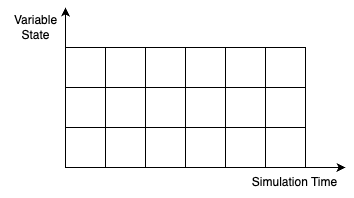
\includegraphics[width=0.7\textwidth]{images/constTime.png}
    \caption{Space-Time Diagram for Time-Stepped Simulation}
    \label{fig:constTime}
\end{figure}

\begin{figure}[H]
    \centering
    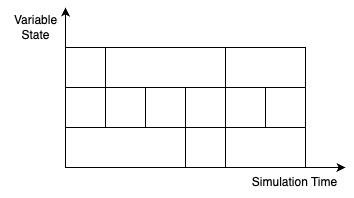
\includegraphics[width=0.7\textwidth]{images/sparseTime.png}
    \caption{Space-Time Diagram for Event-Driven Simulation}
    \label{fig:sparseTime}
\end{figure}

In scenarios where real-time consistency is required, discrete-event simulations can be synchronized to ensure that simulation time progresses in lockstep with real time. This synchronization enables a more cohesive and accurate representation of real-world processes.

\section{Discrete-Event Simulation Framework}

The focus of this work is on discrete-event simulations. A typical DES program relies on three fundamental data structures:

\begin{enumerate}
    \item \textbf{State Variables}: These variables represent the current state of the system.
    \item \textbf{Event List}: A priority queue containing events scheduled to occur at future simulation times, each with a corresponding timestamp.
    \item \textbf{Global Clock Variable}: Represents the current simulation time. If the clock variable has a value $T$, it indicates that all activities up to time $T$ have been simulated, while activities beyond $T$ are yet to be processed.
\end{enumerate}

An event in the DES framework typically consists of a data structure containing its timestamp (e.g., 9:16 AM), event type (e.g., airplane arrival), and various parameters specifying details of the event (e.g., Flight 396 arriving at LAX).

In a physical system, events such as airplane arrivals occur autonomously. In the simulation, however, nothing happens unless an event is explicitly created by the simulation computation. This process is referred to as \textit{event scheduling}. For example, if the simulation reaches time 9:00 and an event indicates that Flight 200 has landed, the simulation can then schedule a new event for this plane’s departure at 9:56. Event scheduling involves allocating memory for a new event, populating its fields (timestamp, event type, and parameters), and adding it to the event list.

\begin{figure}[H]
    \centering
    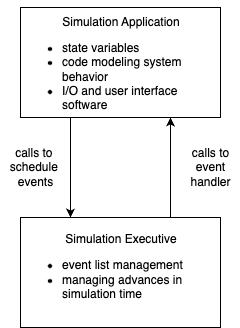
\includegraphics[width=0.4\textwidth]{images/simulationComponents.png}
    \caption{Separation of the Simulation Program into the Simulation Application and Executive Components}
    \label{fig:simComp}
\end{figure}

A discrete-event simulation program can be divided into two major components, as illustrated in Figure~\ref{fig:simComp}:

\begin{itemize}
    \item \textbf{Simulation Executive}: This component maintains the event list and the global clock variable. It operates independently of the specific physical system being simulated, serving as the backbone of the simulation program. Often, it is provided as a generic software library adaptable to simulate various types of systems.
    \item \textbf{Simulation Application}: This component contains the state variables and software routines for modeling the physical system. It is closely tied to the specific characteristics and behaviors of the real-world system being simulated. In its simplest form, the simulation executive must only provide one primitive procedure to the simulation application: a method for scheduling events.
\end{itemize}

The core of the simulation executive is an event-processing loop that repeatedly removes the event with the smallest timestamp from the event list, simulates its occurrence, and advances the simulation clock.


\chapter{Design and Implementation}

\section{System Architecture}

The proposed system is designed based on a Centralized Barrier synchronization model \cite{PaDSS}, where a central entity, referred to as the \textbf{Simulation Executive}, coordinates the synchronization and communication among all other processes in the simulation. Each process interacts with the Simulation Executive to communicate its state and synchronize its progress. When all processes have communicated their current state, the Simulation Executive determines the minimum simulation time that all processes can safely advance to, ensuring consistent progression.

This centralized approach reduces the overall communication overhead significantly. In a typical client-server simulation with $m$ client requests, the number of synchronization messages can reach $O(nm)$, where $n$ is the number of processes, and each request results in at least one `syncSleep(T)` call. Our architecture optimizes this to achieve $O(m)$ synchronization messages by eliminating redundant broadcasts to all processes and instead notifying only the process with the lowest simulation time. The overall system architecture is depicted in Figure~\ref{fig:arch}.

\begin{figure}[H]
    \centering
    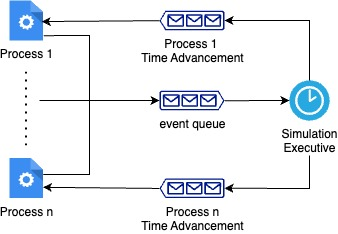
\includegraphics[width=0.7\textwidth]{images/architecture_program.jpg}
    \caption{System Architecture}
    \label{fig:arch}
\end{figure}

Although this approach introduces additional complexity in managing the state of each process, it significantly reduces the number of messages transmitted over the network, leading to an overall performance improvement. At the start of the simulation, each process establishes a connection with the Simulation Executive, creating a dedicated messaging stream. The Simulation Executive handles all connections and disconnections dynamically, ensuring seamless communication and synchronization.

\section{Component Design}

The implementation of the Simulation Executive requires careful consideration of several key components and mechanisms:

\begin{itemize}
    \item \textbf{Event List Management}: Efficient management of the event list is crucial to handle scheduling operations effectively. We employ a priority queue \cite{pqueue} to manage events, allowing insertion and removal of the minimum element in $O(\log n)$ time, where $n$ is the number of events.

    \item \textbf{Managing Simulation Time Advances}: The Simulation Executive must correctly manage the states of all connected processes and handle various edge cases. The simulation time can advance if and only if:

    \begin{center}
        \#\text{list\_management} \\ = \\  n - \#\text{disconnected\_processes} - \#\text{processes\_in\_blocking\_call}
    \end{center}

    This formula ensures that the simulation time advances only when all active processes are ready. Each process in the system can exist in one of the following states:

    \begin{itemize}
        \item \textbf{Running}: The process is actively executing instructions.
        \item \textbf{Sleeping}: The process is waiting in the event list.
        \item \textbf{Blocking}: The process is waiting for a message or response.
        \item \textbf{Disconnected}: The process has left the simulation and is no longer participating.
    \end{itemize}

    To manage these states efficiently, we use an unordered map \cite{umap}, which supports $O(1)$ operations for insertion, deletion, and element counting.
\end{itemize}

\section{Process Interaction Primitives}

The interaction between the processes and the Simulation Executive is facilitated through a set of primitive functions:

\begin{itemize}
    \item \textbf{connect()}: Establishes a connection between a process and the Simulation Executive.
    \item \textbf{alertBlockingCall()}: Notifies the Simulation Executive that the process is waiting for a message or response.
    \item \textbf{exitBlockingCall()}: Notifies the Simulation Executive that the process has exited the blocking state.
    \item \textbf{syncSleep(long double T)}: Signals that the process will resume after a specified simulated time \( T \).
    \item \textbf{mySleep(long double T)}: Emulates real-time sleep, allowing the process to pause for \( T \) time units.
    \item \textbf{disconnect()}: Disconnects the process from the Simulation Executive.
\end{itemize}

Using these primitives, we define the behavior of client, server, and service processes in the simulation. The pseudocode for each process is presented below:

\begin{algorithm}[H]
\caption{Client Behavior Simulation} \label{alg:client_simulation}
\begin{algorithmic}[1]
    \STATE \textbf{Initialize} client parameters.
    \WHILE{True}
        \STATE mySleep(based on the current state)
        \STATE syncSleep(time to send a request)
        \STATE Send a request corresponding to the current state.
        \STATE alertBlockingCall()
        \STATE Wait for the server's response.
        \STATE exitBlockingCall()
        \STATE syncSleep(time to update the state)
        \STATE Update state: $state \leftarrow newState(state)$
    \ENDWHILE
\end{algorithmic}
\end{algorithm}

\begin{algorithm}[H]
\caption{Server Request Handling} \label{alg:server_request_handling}
\begin{algorithmic}[1]
    \STATE \textbf{Initialize} server parameters.
    \WHILE{True}
        \STATE alertBlockingCall()
        \STATE Wait for incoming requests from clients or services.
        \STATE exitBlockingCall()
        \STATE syncSleep(time to process the request)
        \IF{the request is from a client}
            \STATE Forward the request to the corresponding service.
        \ELSE
            \STATE Send the response back to the client.
        \ENDIF
    \ENDWHILE
\end{algorithmic}
\end{algorithm}

\begin{algorithm}[H]
\caption{Service Response Handling} \label{alg:service_response_handling}
\begin{algorithmic}[1]
    \STATE \textbf{Initialize} service parameters.
    \WHILE{True}
        \STATE alertBlockingCall()
        \STATE Wait for requests from the server.
        \STATE exitBlockingCall()
        \STATE syncSleep(time to process the request)
        \STATE Send the response back to the server.
    \ENDWHILE
\end{algorithmic}
\end{algorithm}

\section{Managing Synchronization Issues}

One of the primary challenges in implementing a centralized synchronization model is handling delays caused by network latency. Figure~\ref{fig:IssueImp} illustrates potential synchronization issues when processes transition between different states.

\begin{figure}[H]
    \centering
    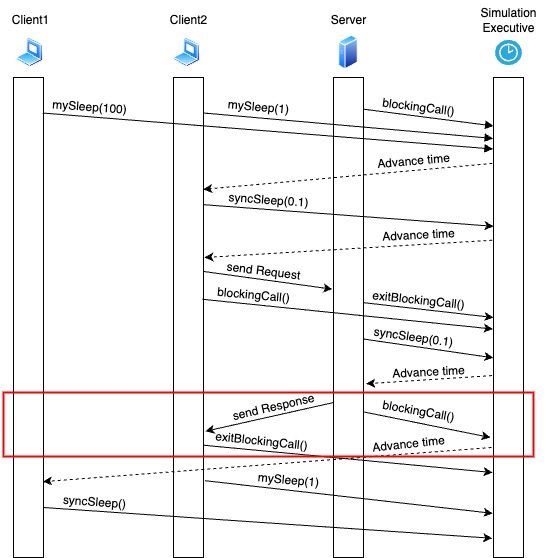
\includegraphics[width=1\linewidth]{images/IssueImp.jpg}
    \caption{Space-Time Diagram of the Simulation}
    \label{fig:IssueImp}
\end{figure}

For instance, after sending a request, `client1` might enter a `Sleeping` state, while `client2` is in a `Blocking` state, waiting for a response from the server. To address these issues, we introduce an additional state:

\begin{itemize}
    \item \textbf{Ready to Exit Blocking Call}: Represents processes that are in a blocking state but are expected to receive a response shortly.
\end{itemize}

To support this state, we define the following additional primitives:

\begin{itemize}
    \item \textbf{sendId(std::string id)}: Associates each process with a unique identifier, facilitating easier tracking of communications.
    \item \textbf{sendingTo(std::string receiverId)}: Notifies the Simulation Executive that a process is sending a message to `receiverId`, allowing it to anticipate a blocking exit.
\end{itemize}

The updated condition for simulation time advancement now becomes:

\begin{center}
    \#\text{list\_management} \\ = \\  n - \#\text{disconnected\_processes} - (\#\text{processes\_in\_blocking\_call} - \#\text{processes\_exiting\_blocking\_call})
\end{center}

This refinement ensures that simulation time advances correctly even under varying network conditions and communication delays.

\subsection*{Simulation Executive}

To start the Simulation Executive, specify the number of processes expected to connect. The executive will then wait for connections to be established with each process before initiating the simulation.

\subsection*{Simulation Application}

The system includes default classes such as `Client`, `Server`, and `Service`, which ensure correct interaction with the Simulation Executive. Custom processes can also be implemented using the described primitives to interact seamlessly with the Simulation Executive, allowing for flexible simulation scenarios, there are also a provided classes that simulate the client based on some inputs, server, and services.


\section{Monitoring and Logging Mechanism}

The system includes two critical components for tracking simulation activities and collecting performance metrics: the \textbf{Simulation Logger} and the \textbf{Performance Monitor}. These components are designed to provide real-time insights into the simulation, detect anomalies, and enable efficient debugging. Such a monitoring architecture follows principles similar to distributed logging systems, which enhance observability and fault detection by aggregating data from multiple sources, thereby offering a comprehensive view of system performance \cite{MediumDistributedLogging}. Figure~\ref{fig:monitors} depicts an illustration of these monitoring mechanisms.

\begin{figure}[H]
    \centering
    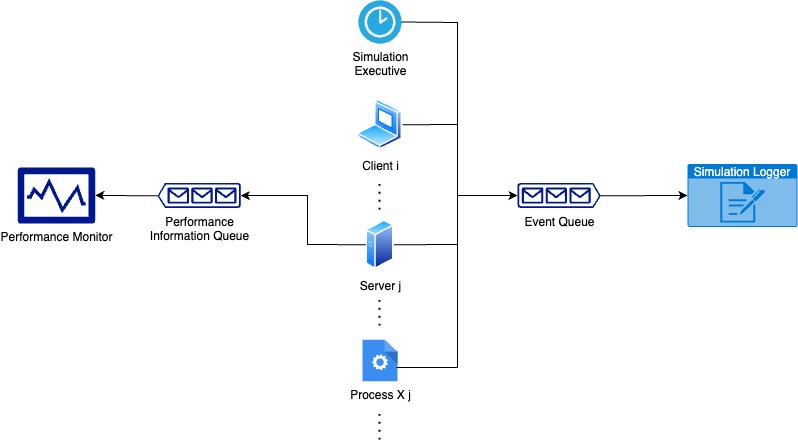
\includegraphics[width=0.7\textwidth]{images/monitors.jpg}
    \caption{Monitoring and Logging Mechanism}
    \label{fig:monitors}
\end{figure}

\subsection{Simulation Logger}

The \textbf{Simulation Logger} records all significant events that occur during the simulation. Each event is logged with the following details:

\begin{itemize}
    \item \textbf{Timestamp}: The timestamp when the event occurred.
    \item \textbf{Event Type}: The type of event (e.g., `connection established`, `alertBlockingCall`, etc.).
    \item \textbf{Stream Name}: The stream where the event originated.
    \item \textbf{Values}: Any associated data relevant to the event.
\end{itemize}

This detailed logging allows for comprehensive post-simulation analysis, facilitating the identification of execution patterns, interactions between processes, and debugging of unexpected behavior.

\subsection{Performance Monitor}

The \textbf{Performance Monitor} collects and analyzes performance metrics during the simulation. It continuously receives data from connected servers and updates key statistics such as:

\begin{itemize}
    \item \textbf{Average Response Time}: The mean response time for all processed requests.
    \item \textbf{Minimum Response Time}: The shortest observed response time.
    \item \textbf{Maximum Response Time}: The longest observed response time.
    \item \textbf{Variance}: The variance in response times, which indicates the consistency of the system's performance.
\end{itemize}

The Performance Monitor not only identifies and alerts users of potential bottlenecks but also allows them to intervene during the simulation. This proactive capability helps in addressing performance issues as they emerge, minimizing disruptions. All performance logs are stored for post-simulation analysis, enabling a comprehensive evaluation of the system's efficiency and facilitating more granular analysis, such as tracing specific inefficiencies or assessing particular scenarios that might have led to performance degradation.



\chapter{Simulation Speed-up}

Understanding the performance gains achieved by utilizing simulated time in a Discrete Event Simulation (DES) model requires a detailed analysis of the cost factors in both real-time and simulated-time scenarios. This chapter explores the key variables influencing system performance and presents formulas to estimate costs and speed-up factors, providing a basis for comparing the efficiency of different simulation techniques.

\section{Key Variables}

To model the simulation's dynamics, the following key variables are defined:

\begin{itemize}
    \item \( p \): The total number of requests initiated by clients throughout the simulation.
    \item \( c \): The number of clients participating in the simulation.
    \item \( n \): The number of possible request types or states a client can have, such as connect, disconnect, or idle.
    \item \( P \): The transition matrix for a Markov chain with dimensions \( n \times n \), representing state transition probabilities that model clients’ behavior.
    \item \( svp \): Stationary distribution vector of the Markov chain, denoted as a \( 1 \times n \) vector, representing the long-term probability distribution of the system’s states.
    \item \( cst \): A vector of dimension \( n \times 1 \) representing the average sleep times of clients in each state.
    \item \( ast \): A vector of dimension \( n \times 1 \) indicating the frequency of send operations performed by clients for each state.
    \item \( art \): A vector of dimension \( n \times 1 \) representing the architecture's average response times for each state.
    \item \( cmot \): A vector of dimension \( n \times 1 \) representing the machine operation times on the client side for each state.
    \item \( amot \): A vector of dimension \( n \times 1 \) representing the architecture's machine operation times for each state.
    \item \( cstoo \): The number of send operations that each client performs to the simulation executive for each request.
    \item \( artoo \): The number of send operations that the architecture performs to the simulation executive for each request.
    \item \( \tau \): The network transmission time, representing the time it takes to send a request over the network.
    \item \( \alpha \): A constant used for scaling time or representing additional delays in specific scenarios.
\end{itemize}

These variables form the basis for calculating the costs in both real-time and simulated-time simulations, allowing for a comprehensive analysis of the speed-up achieved using the simulation framework.

\section{Real-time Simulation Cost}

In real-time simulations, the system operates in synchrony with actual time, meaning that clients follow their defined behavior and sleep periods without any acceleration. The total real-time simulation cost, denoted as \( T_{real} \), can be decomposed into two main components: the time for client operations and the time for architecture operations.

\[
    T_{real} = TClient_{real} + TArchitecture_{real}
\]

The time for client operations \( TClient_{real} \) is given by:

\[
    TClient_{real} = \left\lceil \frac{p}{c} \right\rceil \cdot (svp \cdot cst) + \left\lceil \frac{p}{c} \right\rceil \cdot \tau + \left\lceil \frac{p}{c} \right\rceil \cdot (svp \cdot cmot)
\]

Where:
\begin{itemize}
    \item \( \left\lceil \frac{p}{c} \right\rceil \): The expected number of requests per client.
    \item \( svp \cdot cst \): The expected sleep times for a client, weighted by the stationary distribution vector \( svp \).
    \item \( \tau \): The network transmission time for a client to send a request to the server.
    \item \( svp \cdot cmot \): The expected time spent in machine operations by the client, weighted by the stationary distribution vector.
\end{itemize}

The time for architecture operations \( TArchitecture_{real} \) is given by:

\[
    TArchitecture_{real} = \left\lceil \frac{p}{c} \right\rceil \cdot (svp \cdot art) + \left\lceil \frac{p}{c} \right\rceil \cdot (svp \cdot ast) \cdot \tau + \left\lceil \frac{p}{c} \right\rceil \cdot (svp \cdot amot)
\]

Where:
\begin{itemize}
    \item \( svp \cdot art \): The expected server processing time for each request, weighted by the stationary distribution vector \( svp \).
    \item \( (svp \cdot ast) \cdot \tau \): The network time for sending responses to clients, where \( ast \) is the vector indicating the frequency of send operations based on the state.
    \item \( svp \cdot amot \): The expected time spent in machine operations by the architecture, weighted by the stationary distribution vector.
\end{itemize}

\section{Simulated-time Simulation Cost}

In simulated-time simulations, the system operates based on simulated time, skipping idle periods and thereby accelerating the simulation process. The total simulated-time simulation cost, denoted as \( T_{simulated} \), can be broken down into three main components: the time for client operations, the time for architecture operations, and the time for simulation executive operations.

\[
    T_{simulated} = TClient_{simulated} + TArchitecture_{simulated} + TSimExecutive_{simulated}
\]

The time for client operations \( TClient_{simulated} \) is given by:

\[
    TClient_{simulated} = (svp \cdot cstoo) \cdot p \cdot \tau + p \cdot \tau + p \cdot (svp \cdot cmot)
\]

Where:
\begin{itemize}
    \item \( (svp \cdot cstoo) \cdot p \cdot \tau \): The total network time for messages from clients to the simulation executive, considering the number of requests \( p \) and the network transmission time \( \tau \).
    \item \( p \cdot \tau \): The network time for sending requests to the server.
    \item \( p \cdot (svp \cdot cmot) \): The time spent in machine operations by the clients.
\end{itemize}

The time for architecture operations \( TArchitecture_{simulated} \) is given by:

\[
    TArchitecture_{simulated} = (svp \cdot artoo) \cdot p \cdot \tau + p \cdot (svp \cdot ast) \cdot \tau + p \cdot (svp \cdot amot)
\]

Where:
\begin{itemize}
    \item \( (svp \cdot artoo) \cdot p \cdot \tau \): The total network time for messages from the architecture to the simulation executive.
    \item \( p \cdot (svp \cdot ast) \cdot \tau \): The network time for sending responses to clients and internal messages within the architecture.
    \item \( p \cdot (svp \cdot amot) \): The time spent in machine operations by the architecture.
\end{itemize}

The time for simulation executive operations \( TSimExecutive_{simulated} \) is given by:

\[
    TSimExecutive_{simulated} = (svp \cdot (cstoo + artoo)) \cdot p \cdot \theta + p \cdot (\beta + \tau)
\]

Where:
\begin{itemize}
    \item \( (svp \cdot (cstoo + artoo)) \cdot p \cdot \theta \): The processing time of a request by the simulation executive, considering the combined send operations of clients and the architecture.
    \item \( p \cdot (\beta + \tau) \): The time to resolve synchronization and network delays in the system.
\end{itemize}

\section{Simulation Speed-up Factor}

The speed-up factor \( SimulationSpeedUp \) achieved by using simulated time can be estimated as:

\[
SimulationSpeedUp = \frac{T_{real}}{T_{simulated}}
\]

This ratio quantifies the extent to which the simulation runs faster by utilizing simulated time, eliminating idle periods, and optimizing request handling through the simulation executive.


\chapter{Validation}

\section{Problem Description }

We aim to design and implement a new e-commerce system in this scenario. Based on business studies, the expected number of clients and their behavior are defined. The goal is to evaluate different architectural designs against non-functional requirements, particularly focusing on performance. The architecture team is exploring how many replications of the architecture they need to know how many replications need to satisfy the performance requirements.

\begin{figure}[H]
    \centering
    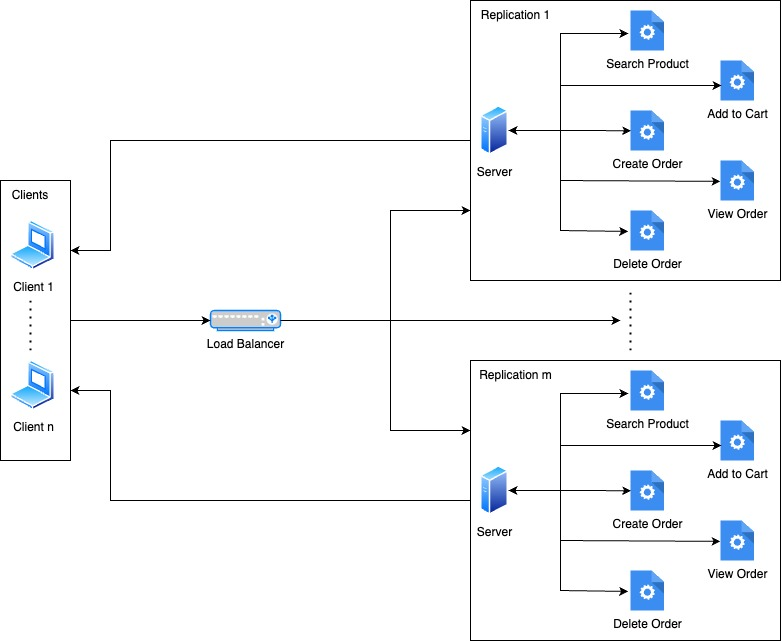
\includegraphics[width=1\linewidth]{images/archEcom.jpg}
    \caption{Eccomerce Software Design}
    \label{fig:eds}
\end{figure}

Line you can see, the architecture \ref{fig:eds} is divided in $m$ replication, and there is also a load balance \cite{loadBalancer} that will just randomacaly make connect a client to the server of a replication, than the client can make some requests based on their behaviour implemented with a markov chain \cite{markovChain}, also the load balancer can be considered as a DNS load Balancer.
\\ \\
And to define the behavior of the customer we can use a markov chain \ref{fig:markovchain}

\begin{figure}[H]
    \centering
    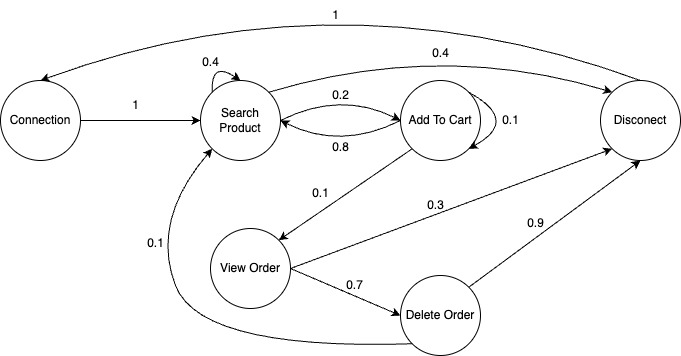
\includegraphics[width=\textwidth]{images/markovchain.jpg}
    \caption{Customer behaviour though Markov chain}
    \label{fig:markovchain}
\end{figure}


Now let's define the variables that will allow us to do the simulation and define the $SpeedUpSimulation$:
\begin{itemize}
    \item \( P = \begin{bmatrix}
                0 & 1 & 0 & 0 & 0 & 0 \\ 
                0 & 0.4 & 0.2 & 0 & 0 & 0.4 \\ 
                0 & 0.8 & 0.1 & 0.1 & 0 & 0 \\ 
                0 & 0 & 0 & 0 & 0.7 & 0.3 \\
                0 & 0.1 & 0 & 0 & 0 & 0.9 \\ 
                1 & 0 & 0 & 0 & 0 & 0
            \end{bmatrix} \)
    
    %\item \( svp = \begin{bmatrix} 0.20019036 & 0.47588832 & 0.10575296 & 0.0105753 & 0.00740271 & 0.20019036 \end{bmatrix} \)
    
    \item \( cst = \begin{bmatrix} 5 \times 86400 & 20 \times 60 & 16 \times 60 & 20 \times 60 & 1 \times 60 & 3600 \end{bmatrix}^{T} \)
    
    \item \( ast = \begin{bmatrix} 1 & 3 & 3 & 3 & 3 & 0 \end{bmatrix}^{T} \) 
    
    \item \( art = \begin{bmatrix} 0.3 & 0.7 & 0.4 & 0.5 & 0.4 & 0.1 \end{bmatrix}^{T} \)
    
    \item \( cmot = \begin{bmatrix} 10^{-7} & 10^{-7} & 10^{-7} & 10^{-7} & 10^{-7} & 10^{-7} \end{bmatrix}^{T} \)
    
    \item \( amot = \begin{bmatrix} 2 \times 10^{-7} & 2 \times 10^{-7} & 2 \times 10^{-7} & 2 \times 10^{-7} & 2 \times 10^{-7} & 2 \times 10^{-7} \end{bmatrix}^{T} \)
    
    \item \( network\_cost = 0.00023 \)
    
    \item \( cstoo = \begin{bmatrix} 4 & 3 & 3 & 3 & 3 & 1 \end{bmatrix}^{T} \)
    
    \item \( artoo = \begin{bmatrix} 3 & 9 & 9 & 9 & 9 & 2 \end{bmatrix}^{T} \)
    
    \item \( \theta = 5 \times 10^{-7} \)
    
    \item \( \beta = 1 \times 10^{-7} \)
    
    \item \( \alpha = 30 \)
\end{itemize}



\section{Non-functional Requirements}

Non-functional requirements (NFRs) define the quality attributes of a system, and they are critical for evaluating its performance, reliability, and maintainability. 
To 

Here, we will outline the key NFRs for our system, focusing on how they can be measured and how our simulation tool helps ensure performance qualities.

\begin{table}[H]
    \centering
    \small
    \renewcommand{\arraystretch}{1.5}
    \begin{tabular}{|c|c|c|c|c|}
        \hline
        \textbf{Server ID} & \textbf{Request Type} & \textbf{Request Time} & \textbf{Read Request} & \textbf{Response Time} \\
        \hline
        2100 & connection & 322.896095 & 322.896325 & 322.896555 \\
        \hline
        2100 & connection & 734.715306 & 734.715536 & 734.715766 \\
        \hline
        2100 & searchProduct & 966.871627 & 966.871857 & 967.572547 \\
        \hline
        2100 & searchProduct & 1066.145295 & 1066.145525 & 1066.846215 \\
        \hline
        2100 & searchProduct & 1432.340573 & 1432.340803 & 1433.041493 \\
        \hline
    \end{tabular}
    \caption{Request times and responses.}
    \label{tab:request_times}
\end{table}


Using the log structure (Table~\ref{tab:request_times}), we can calculate important metrics like minimum, maximum, mean, and variance for each request type, allowing us to assess the overall performance. These metrics give us insights into various NFRs, as explained below.

\subsection{Performance Metrics}

Performance is often the most critical non-functional requirement in systems handling large amounts of requests, as in our e-commerce scenario. We can calculate several performance-related metrics such as:

\begin{itemize}
    \item \textbf{Latency}: Time taken to process a request, measured from the logs.
    \item \textbf{Min, Max, Mean, and Variance}: Statistical measures to track response times, helping to identify performance bottlenecks.
\end{itemize}

\begin{table}[h!]
    \centering
    \renewcommand{\arraystretch}{1.5}
    \resizebox{!}{0.11\textwidth}{ % Adjust the height value (0.5\textheight) to compress vertically
        \begin{tabular}{|c|c|c|c|c|c|c|}
            \hline
            \textbf{Request Type} & \textbf{Min Request} & \textbf{Max Request} & \textbf{Mean Request} & \textbf{Var Request} & \textbf{Count Requests} \\
            \hline
            addToCart & 0.40092 & 0.630819 & 0.400996 & 1.745494e-05 & 3028 \\
            \hline
            connection & 0.00046 & 0.000460 & 0.000460 & 1.970162e-21 & 6539 \\
            \hline
            createOrder & 0.50092 & 0.500920 & 0.500920 & 2.117974e-21 & 300 \\
            \hline
            searchProduct & 0.70092 & 1.482193 & 0.702789 & 8.150574e-04 & 14197 \\
            \hline
            viewOrder & 0.40092 & 0.400920 & 0.400920 & 4.094827e-21 & 207 \\
            \hline
        \end{tabular}
    }
    \caption{Non-functional requirements results: Performance Analysis}
    \label{tab:request_statistics}
\end{table}


\subsection{Results and Observations}

We conducted tests with a range of values for \( p \) (number of client requests) and different values for \( c \) (number of clients), observing the simulation speed-up, \( SimulationSpeedup \). The goal is to determine when it is more convenient to use simulated-time simulations and when real-time simulations might be more efficient.

\begin{figure}[H]
    \centering
    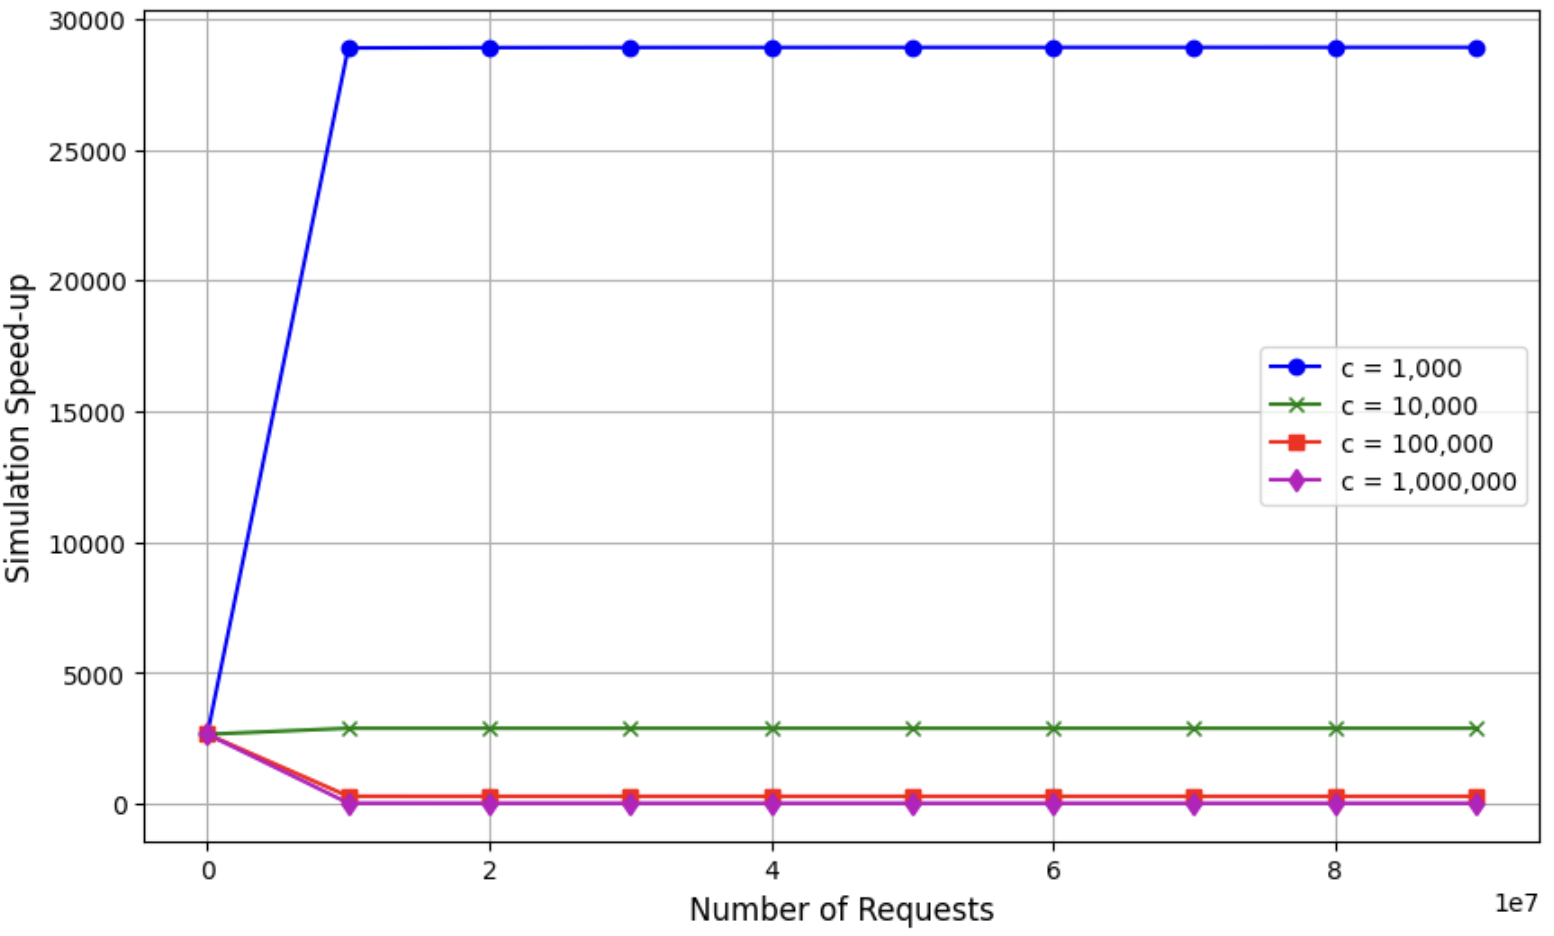
\includegraphics[width=\textwidth]{images/speed-up_result.png}
    \caption{Performance ratio}
    \label{fig:performance_ratio}
\end{figure}

Considering different values of \( c \) (number of clients), we observe that the simulation speed-up is significantly higher when the number of clients (\( c \)), is lower. This behavior is due to the parallel processing advantage of real-time simulations being less pronounced when there are fewer processes. With a lower number of clients, the overhead of coordinating real-time operations diminishes, making simulated time more efficient.

As the number of clients, \( c \), increases, real-time simulations become more efficient, and the total simulated time, \( T_{simulated} \), remains relatively unchanged. This is because real-time simulations can better distribute the workload across multiple machines.

Now lets' do see better if it's better than having a 10 times faster then real time\ref{fig:perfZoom}

\begin{figure}[H]
    \centering
    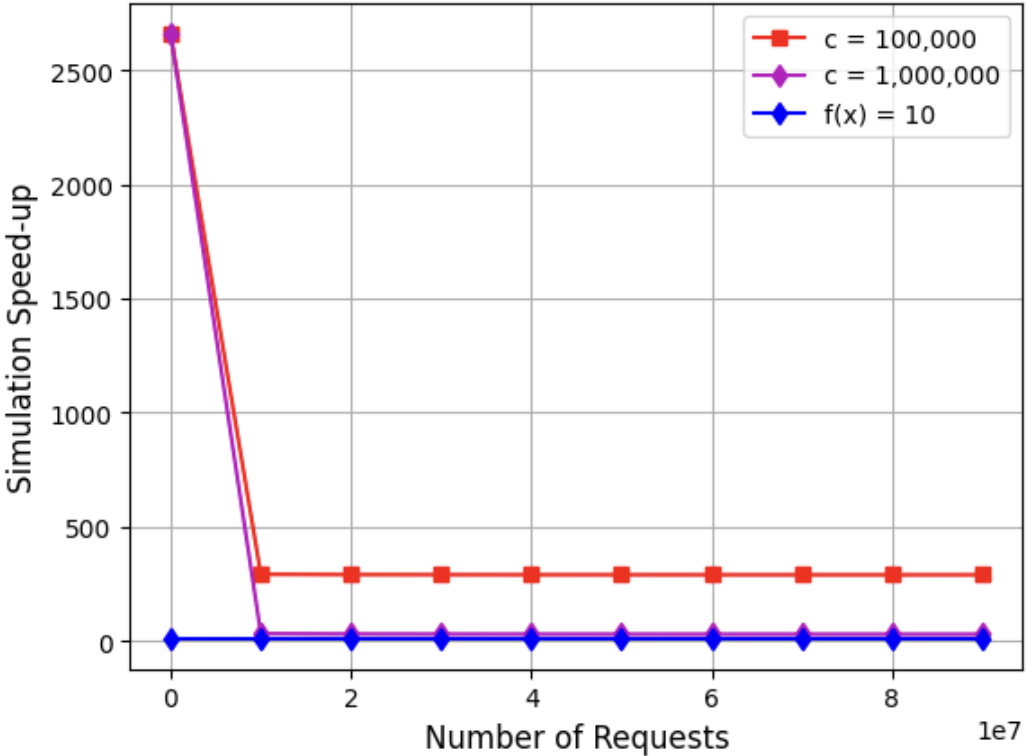
\includegraphics[width=\textwidth]{images/zoomgraph.png}
    \caption{Zoom on function with lower $SimulationSpeedUp$}
    \label{fig:perfZoom}
\end{figure}


We also sought to determine the maximum number of clients \( c \) that can handle at least 100,000,000 requests (\( p \)) while achieving a \( SimulationSpeedup \geq 10 \). Our findings indicate that \( c = 2,941,176 \) is required to achieve a speed-up of 10x in this scenario.



\chapter{Validation of Formula Results}

\section{Methodology for Validation}

Validating the proposed formulas for computing simulation time (\( T_{simulated} \)) is a critical step to ensure their reliability and applicability. While the formula for real-time execution (\( T_{real} \)) does not require further validation—since it directly reflects the time elapsed during real-world execution with actual delays—the simulated time formulas need rigorous testing to verify their accuracy.

To validate \( T_{simulated} \), a series of experiments were conducted using various configurations of \( p \) (number of requests) and \( c \) (number of clients). The simulation results obtained from the tool were then compared against the theoretical values predicted by our formulas. This comparison was performed by measuring the actual time taken to execute the simulated test cases and calculating the percentage error between the observed and predicted values.

\subsection{Test Setup and Experimental Design}

The experiments were designed to evaluate the formulas across a range of scenarios with varying numbers of clients and requests. Each configuration was executed multiple times to account for variability in results due to system performance or environmental factors. The following test configurations were used:

\begin{itemize}
    \item \textbf{Number of Requests (\( p \))}: 10,000, 20,000, and 30,000.
    \item \textbf{Number of Clients (\( c \))}: 100, 500, and 1,000.
\end{itemize}

The system under test was executed on a single machine, with the simulation tool configured to use the same settings for all runs. The predicted time values were computed based on the derived formulas, and the actual simulation times were recorded for each configuration.

For clarity, we define \( T_{real} \) as the time measured for the actual implementation of the system, and \( T_{simulated} \) as the value computed using our formulas.

\section{Error Analysis and Accuracy Metrics}

To quantify the accuracy of the simulation results compared to the predicted values, the following formula was used to calculate the percentage error:

\[
    \text{Error} = \frac{|T_{predicted} - T_{simulated}|}{T_{predicted}} \times 100
\]

This error metric provides a measure of the deviation between the theoretical and experimental results, helping identify the scenarios where our formulas closely approximate the actual simulation time and where deviations occur. A lower error percentage indicates that the formulas are highly accurate, while a higher percentage suggests potential inefficiencies or inaccuracies in either the formula or the simulation model.

\subsection{Analysis of Results}

The results show that the formula for \( T_{simulated} \) provides an accurate approximation of the actual simulation time in most cases. However, as the number of clients (\( c \)) increases, the error tends to rise slightly. This is likely due to the increased computational overhead of managing a larger number of processes in a single-machine environment. The kernel’s scheduling and context-switching operations introduce additional delays not captured by the formulas, which assume an idealized processing scenario.

The experimental results are summarized in Table \ref{table:validation_results}, which presents the predicted and actual simulation times, along with the calculated error percentages for each configuration.

\begin{table}[h!]
    \centering
    \resizebox{0.85\textwidth}{!}{
    \begin{tabular}{|c|c|c|c|c|}
    \hline
    \textbf{Requests} & \textbf{Clients} & \textbf{$T_{predicted}$ (sec)} & \textbf{$T_{simulation}$ (sec)} & \textbf{Error (\%)} \\ \hline
    10,000 & 100  & 60.40 & 58 & 3.97\% \\ \hline
    10,000 & 500  & 60.40 & 61 & 0.99\% \\ \hline
    10,000 & 1,000 & 60.40 & 62 & 2.64\% \\ \hline
    20,000 & 100  & 90.80 & 87 & 4.18\% \\ \hline
    20,000 & 500  & 90.80 & 90 & 0.88\%  \\ \hline
    20,000 & 1,000 & 90.80 & 91 & 0.22\%  \\ \hline
    30,000 & 100  & 121.20 & 114 & 5.94\% \\ \hline
    30,000 & 500  & 121.20 & 118 & 2.64\% \\ \hline
    30,000 & 1,000 & 121.20 & 122 & 0.66\% \\ \hline
    \end{tabular}
    }
    \caption{Comparison of predicted and actual simulation times for varying numbers of requests and clients}
    \label{table:validation_results}
\end{table}

\subsection{Interpretation of Results}

The results in Table \ref{table:validation_results} demonstrate that the formulas for \( T_{simulated} \) perform well under most conditions, with an average error of less than 3\% across all configurations. The highest error was observed for 30,000 requests and 100 clients, where the percentage error reached 5.94\%. This suggests that the formula’s accuracy may decrease slightly under higher loads when the number of clients is relatively small compared to the number of requests.

One possible explanation for this discrepancy is the impact of process management overhead, which is more pronounced when a small number of clients handle a large volume of requests. In such cases, the overhead introduced by context switching and I/O operations can lead to increased execution time, which is not accounted for in the simplified formulas used to derive \( T_{simulated} \).
\\ \\
The validation of the formulas for \( T_{simulated} \) confirms that they provide an accurate approximation of actual simulation times under a variety of configurations. While the formulas maintain high accuracy in most cases, further refinement may be needed to account for system-specific factors such as process management overhead and resource contention. Future work will focus on enhancing the formulas to incorporate these factors, improving the precision of simulation time predictions in complex scenarios.

Overall, the results demonstrate that the proposed approach is effective in estimating simulation times, enabling developers and architects to perform quick, reliable validations of system performance without the need to run exhaustive real-time tests.


\chapter{Conclusion and Future Work}

In this thesis, we successfully designed and validated a new e-commerce system architecture focused on meeting essential non-functional requirements, particularly performance. Through rigorous experimentation and simulation, we established a framework to evaluate various architectural designs against expected client behavior, ultimately enhancing our understanding of how system performance can be optimized.

\section{Summary of Results}

The results demonstrated that our proposed architecture, characterized by multiple server replications and a DNS-based load balancer, effectively managed client requests. By employing a Markov chain to simulate customer interactions, we were able to capture the dynamic nature of user behavior and its impact on system performance. Key performance metrics, including latency, response times, and overall simulation speed-up, were analyzed under various configurations of clients and requests. 

Notably, we observed that simulated-time simulations yielded significant speed-ups when the number of clients was limited, while real-time simulations became more efficient as client numbers increased. This insight allows architects and developers to strategically select testing methodologies based on system load, ultimately enhancing testing efficiency and reliability.

Additionally, our research established that achieving a target of 100 million requests with a speed-up of at least 10x necessitates approximately 2.9 million clients. This finding underscores the scalability potential of our architecture and emphasizes the importance of load management in high-demand scenarios.

\section{Future Work}

Despite the significant contributions of this research, several areas warrant further exploration to enhance the robustness and applicability of our findings:

\begin{itemize}
    \item \textbf{Advanced Load Balancing Techniques:} Future work could investigate alternative load-balancing algorithms that adapt dynamically to changing workloads and client behaviors. This would improve resource allocation and further optimize response times.

    \item \textbf{Incorporation of Additional Non-Functional Requirements:} While this thesis focused primarily on performance, extending the analysis to include other non-functional requirements such as reliability, scalability, and security could provide a more comprehensive evaluation of the system's capabilities.

    \item \textbf{Longitudinal Studies:} Conducting long-term performance assessments in real-world environments would help validate our simulation results and uncover any unforeseen issues that arise under sustained loads.

    \item \textbf{Multi-Cloud Deployments:} As cloud computing continues to evolve, examining the effects of deploying this architecture across multiple cloud platforms could provide insights into optimizing costs and performance while maintaining high availability.
\end{itemize}

\section{Conclusion}

In conclusion, this research successfully validated a novel e-commerce system architecture that meets crucial performance requirements through simulation and analysis. The insights gained from our experiments serve as a foundation for further developments in e-commerce systems, paving the way for more efficient architectures capable of handling increasing demand. By addressing the outlined future work, we can enhance the adaptability and robustness of our system, ensuring its relevance in the fast-paced landscape of digital commerce.


\chapter*{Acknowledgments}

What started as an unexpected detour has now led me to this final chapter of my bachelor’s degree. It’s been a challenging journey, full of surprises, but I’m finally here.

First and foremost, I would like to express my deepest gratitude to my advisor, who always made himself available, and to my co-advisor for introducing me to this project.

I am profoundly grateful to my parents for their unwavering support, belief in my potential, and their sacrifices throughout this path, allowing me to pursue my own way and follow my aspirations.

To my university classmates, with whom I spent most of these years, thank you for the countless hours we shared, helping me grow not just technically but, more importantly, as a person.

To my closest friends, who have been there since kindergarten and middle school, thank you for being a source of comfort and for helping me take breaks from university life. Your support has meant the world to me.

Finally, I want to thank everyone who has helped me grow. Your support has made all the difference. 


\backmatter


\phantomsection
\begin{thebibliography}{17}

\bibitem{shadowTestingMicrosoft}
Microsoft. Shadow Testing in Automated Testing. Available online: \url{https://microsoft.github.io/code-with-engineering-playbook/automated-testing/shadow-testing/}.

\bibitem{PaDSS} 
    R. M. Fujimoto, \textit{Parallel and Distributed Simulation Systems}. Wiley-Interscience, 2000.

\bibitem{pqueue}
cppreference.com contributors, 
\emph{std::priority\_queue}. 
Available: \url{https://en.cppreference.com/w/cpp/container/priority_queue}.

\bibitem{bigO}
Wikipedia contributors, "Big O notation", \textit{Wikipedia, The Free Encyclopedia}, Available at: \url{https://en.wikipedia.org/wiki/Big_O_notation}

\bibitem{umap}
cppreference.com contributors, 
\emph{std::unordered\_map}. 
Available: \url{https://en.cppreference.com/w/cpp/container/unordered_map}.

\bibitem{nprs}
Wikipedia contributors, "Non-functional requirement", \textit{Wikipedia, The Free Encyclopedia}, Available at: 
\url{https://en.wikipedia.org/wiki/Non-functional_requirement}

\bibitem{loadBalancer}
Amazon Web Services, Inc. \textit{What is Load Balancing?}. Available at: \url{https://aws.amazon.com/it/what-is/load-balancing/}.

\bibitem{markovChain}
J. D. Herniter and J. F. Magee, ``Customer Behavior as a Markov Process,'' \textit{Operations Research}, vol. 9, no. 1, pp. 105-122, Jan. - Feb., 1961.

\bibitem{stationary}
``MathWorks, ``Markov Chain Analysis and Stationary Distribution,'' [Online]. Available: \url{https://it.mathworks.com/help/symbolic/markov-chain-analysis-and-stationary-distribution.html}.

\bibitem{MediumDistributedLogging}
Vaishnavi Abirami,
\textit{Mastering Microservices Logging - Best Practices Guide},
August 29, 2024. Available: \url{https://signoz.io/blog/microservices-logging/}


\end{thebibliography}

\end{document}